\documentclass[12pt, a4paper]{article}
\usepackage[magyar]{babel}
\usepackage[T1]{fontenc}
\usepackage[margin=2.5cm]{geometry}
\usepackage{amsmath}
\usepackage{amssymb}
\usepackage{graphicx}
\usepackage{float}


\title{\bfseries Lézerfizika tételsor}
\author{Illés Gergő, Sarkadi Balázs}
\begin{document}
\maketitle

\section{Mit rövidít a ,,laser'' mozaikszó?}
\textbf Light \textbf Amplification by \textbf Stimulated \textbf Emission of \textbf Radiation.

\section{Min alapszik a mátrixokkal való sugárkövetés (mátrixoptika)?}
A mátrixoptikai leírásban a sugarakat 2 paraméterrel jellemezzük. Az optikai tengelytől való távolsággal és az optikai tengellyel bezárt szöggel. Továbbá paraxiális közelítésben vagyunk ami azt jelenti, hogy a szögek szinuszait magával a szög értékével közelítjük. Egyes optikai elrendezést úgynevezett sugártranszfer (ABCD) mátrixszal jellemezhetünk, ami a következő egyenletrendszert kódolja.
\begin{equation}
\begin{pmatrix}
A&B\\C&D
\end{pmatrix}\cdot
\begin{pmatrix}
x_1\\\varphi_1
\end{pmatrix}=\begin{pmatrix}
x_2\\\varphi_2
\end{pmatrix}
\end{equation}

\section{Adja meg $f$ fókusztávolságú vékony lencse és $d$ távolságon való terjedés mátrixait!}
\begin{equation}
\begin{pmatrix}
1&0\\-\frac{1}{f}&1
\end{pmatrix}\;\text{és}\;
\begin{pmatrix}
1&d\\0&1
\end{pmatrix}
\end{equation}

\section{Adja meg az optikai rezonátor stabilitási feltételét!}
\begin{equation}
0\leq\left(1-\frac{L}{R_1}\right)\left(1-\frac{L}{R_2}\right)\leq 1
\end{equation}
\begin{equation}
0 \leq \frac{A+D+2}{4} \leq 1
\end{equation}

\section{Határozza meg a Gauss-nyalábok átmérőjét és görbületi sugarát adott helyen a nyalábnyak és a hullámhossz függvényében!}
\begin{align}
W(z) &= w_0\cdot\sqrt{1+\left(\frac{z}{z_R}\right)^2}\\
R(z) &= z\cdot\left[1+\left(\frac{z_R}{z}\right)^2\right]\\
z_R &= \frac{nw_0^2\pi}{\lambda}
\end{align}

\section{Definiálja a Gauss nyalábokra felírható komplex nyaláb paramétert! Adja meg, hogy az 1-es számú síkban felvett $q_1$ hogyan viszonyol a 2-es síkban felvett $q_2$-höz!}
\begin{align}
q(z) &= z+iz_R\\
q_2 &= \frac{Aq_1+B}{Cq_1+D}
\end{align}

\section{Mekkora a frekvenciakülönbség egy L hosszúságú rezonátorban kialakuló módusok közötti frekvenciakülönbség?}
\begin{equation}
\Delta f = \frac{c}{2L}
\end{equation}

\section{Mi az összefüggés a foton élettartama ($\tau_p$), a körülfordulási idő($\tau_{RT}$) és a ,,túlélési faktor'' ($S$) között? Mi az összefüggés a foton élettartam és ($Q$) minőségi faktor között?}
\begin{align}
\tau_p &= \frac{\tau_{RT}}{1-S}\\
\tau_p &= \frac{Q}{\omega_0}
\end{align}

\section{Definiálja Einstein szerinti leírásban lévő $B_{12}$ abszorpciós, $B_{21}$ kényszerített emissziós és $A_{21}$ spontán emissziós együtthatót!}
\begin{align}
\left.\frac{dN_2}{dt}\right\vert_{sp.e.}&=-A_{21}\cdot N_2\\
\left.\frac{dN_2}{dt}\right\vert_{st.e.}&=-B_{21}\cdot N_2\cdot \rho(\nu)\\
\left.\frac{dN_2}{dt}\right\vert_{abs.}&=B_{12}\cdot N_1\cdot \rho(\nu)\\
\frac{N_2}{N_1}&=\frac{B_{12}\cdot\rho(\nu)}{A_{21}+B_{21}\cdot\rho(\nu)}\\
g_2 B_{21} = g_1 B_{12} \hspace{0.5cm} & \hspace{0.5cm} \frac{A_{21}}{B_{21}} = \frac{8 \pi n^2 n_g h \nu^3}{c^3}
\end{align}

\section{Hogy viszonyulnak egymáshoz a kényszerített emisszió által kibocsátott és az azt kiváltó foton tulajdonságai?}
Frekvencia, polarizáció, fázis és haladási irány megegyezik.

\section{Definiálja a hatáskeresztmetszet empirikus jelentését!}
A hatáskeresztmetszet a részecske olyan környezete ahol a fotonokkal interakcióba léphet.

\vspace{0.5cm}Másképp:

Effektív terület vagy valószínűség abszorpcióra vagy foton emisszióra egy adott energia szinten. 

\vspace{0.5cm}Harmadképp:

Interakció valószínűsége az atom/molekula/ion és a beeső sugárzás között.

\section{Adja meg az összefüggést az erősítési együttható, az emissziós és abszorpciós hatáskeresztmetszetek és populációk közti összefüggést adott energiaszinten!}
\begin{equation}
\gamma(\nu)=N_2\sigma_{em}(\nu)-N_1\sigma_{abs}(\nu)
\end{equation}

\section{Írja fel egy három szintű lézer populációváltozásának egyenleteit s hatáskeresztmetszetek segítségével!}
(0-2 pumpa, 2-1 spontán emissziós, 1-0 stimulált emisszió?)

Csak a sugárzással járó átmeneteket figyelembe véve:
\begin{center}
\begin{align}
\frac{dN2}{dt} &= \sigma_{abs} N_0 - \frac{N_2}{\tau_{p2}}\\
\frac{dN1}{dt} &= \frac{N_2}{\tau_{p2}} - \frac{N_1}{\tau_{p1}} - \sigma_{em} N_1\\
N &= N_0 + N_1 + N_2 \text{\hspace{2 cm}, ahol N konstans}
\end{align}
\end{center}


\section{Mi a spektrális kiszélesedés két fajtája? Mi a különbség az abszorpciós vagy emissziós szaturációban? (ellenőrizni)}
1, Homogén kiszélesedés: Az erősítési térben lévő részecskék energia szintjei közötti különbség azonos. Több frekvencia komponens vesz részt az erősítésben abszorbens anyag jelenlétében ezáltal a szaturáció jelentősebb mértékű\\
2, Inhomogén kiszélesedés: égethető\\
Az erősítési térben a részecskék energiaszintjei közötti különbségek nem teljesen egyformák, így a kiszélesedés struktúrált lehet, ezáltal kevesebb frekvencia komponens vesz részt az erősítésben abszorbens anyag jelenlétében így a szaturáció mértéke is csökken.

\section{Mit jelent a Q-kapcsolás? Mekkora a Q-kapcsolt lézerek impulzushossza? Hogyan viszonyul ez a körülfutási időhöz?}
A Q-kapcsolás lényege az, hogy pumpálás alatt megnöveljük a rezonátorban lévő veszteséget, így az erősítés alacsony lesz és nagyon sok részecskét tudunk gerjesztett állapotba juttatni, mivel a spontán kibocsátott fotonok nem erősödnek jelentősen. Ezután a veszteséget lecsökkentjük, ilyenkor a spontán emisszió jele nagyon gyorsan nagy mértékeben megnő. Ezzel nagyenergiájú rövid impulzusokat hozhatunk létre. Könyv: körüljárási idő: $\approx 1,75$ ns, impulzushossz: $\approx 7,1$ ns tehát nagyjából 5 körülfutás.

\section{Mi a módusszinkronizált lézer? Tipikusan milyen hullámhosszon működtethetőek? Hogyan viszonyul az impulzushossz a körülfutási időhöz?}
A lézertérben különböző longitudinális hullámok alakulhatnak ki, (tegyük fel) azonos amplitúdóval és véletlenszerű fázissal, ezzel egy periodikusan változó intenzitás lefutású impulzust kapunk. Módusszinkronizálásnak nevezzük azt amikor ezekből a módusokból csak bizonyos módusokat erősítünk. Ehhez plusz eszközöket telepítünk a rezonátorba.

\begin{figure}[H]
\center
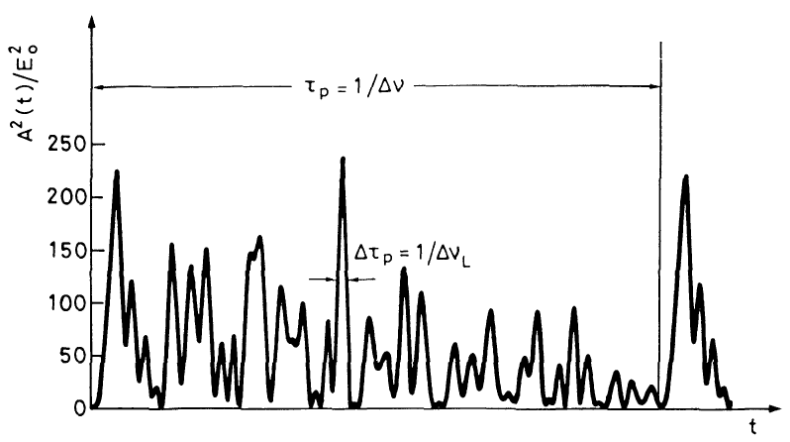
\includegraphics[width=0.5\textwidth]{longitudinalModes}
\caption{Azonos amplitúdójú és véletlenszerű fázissal rezgő longitudinális módusok összege.}
\end{figure}

\underline{Aktív módusszinkronizálásról} beszélünk, amikor ezt a szelekciót egy kívülről vezérelt berendezéssel tesszük meg. Pl egy idővezérelt kapuval a véletlenszerűen keletkező (de periodikusan állandó intenzitás lefutású) impulzus csak egy kiválasztott részét csatoljuk ki mindig a lézerből ($\frac{2L}{c}$ időközönként) ezzel megrövidítve az eredeti impulzust.

\underline{Passzív módusszinkronizálásról} beszélünk, amikor a rezonátorba egy telítődő abszorpens anyagot helyezünk el, ami a nagyobb intenzitású sugárzás hatására gyorsan átlátszóvá válik (azt átengedve), a véletlen amplitúdójú hullám többi részét viszont kiszűri, így csak azokat a módusokat erősítjük, amikre szükségünk van és így rövidebb impulzusokat kaphatunk.

Impulzushossz: ps - fs tartományban működnek jellemzően. Körüljárási idő: 1-10 ps.

\section{Nevezzen meg két gázlézert és két szilárdtest lézert! Írja le az ezekre jellemző paramétereket!}
Gázlézerek:
\begin{enumerate}
\item HeNe: 5:1-től egészen 20:1 arányban tartalmaz héliumot és neont. A tipikus belső nyomás 1 torr (133 Pa). $\lambda$=632.8 nm. Folytonos üzemű. 50 mW optikai teljesítmény.
\item CO$_2$: $\lambda$=10.6 $\mu$m, legrövidebb impulzushossz $\sim$2 ps. Folytonos teljesítménye maximálisan 100 kW nagyságrendű, impulzus üzem esetén GW nagyságrendű
\end{enumerate}	
Szilárdtest lézerek:	
\begin{enumerate}
\item Ti:Sapphire: hangolható 650- és 1100 nm között, általában 800 nm. Al$_2$O$_3$ Ti$^{3+}$ ionokkal szennyezve. Legrövidebb impulzushossz $\sim$10 fs. Folytonos teljesítménye max $\sim$ 2,5 W.
\item Nd:YAG: anyaga: Nd:Y$_3$Al$_5$O$_{12}$. Frekvenciák 946-, 1120-, 1320-, 
\end{enumerate}

\section{Hogyan épül fel egy Szabad elektron Lézer (FEL)? Milyen összefüggés van a FEL sugárzási hullámhossza ($\lambda$), az undulátor periodus hossza ($\Lambda$), a wiggler konstans ($a_w$) és a Lorentz Faktor ($\gamma$) között?}
A szabadelektron lézerek általában egy lineáris gyorsító szakaszból (több lineáris gyorsító egymás után) és egy undulátor szakaszból áll (szintén több darab van egymás után). A lineáris gyorsítóban az elektronokat relativisztikus sebességre (v $\sim$ c) gyorsítják, amiket átvezetnek az undulátorba, ami egy periodikusan kialakított mágneses teret hoz létre, amiben az elektronok egy szinuszra emlékeztető pályán haladnak. Ennek következtében sugárzás keltődik a folyamatos gyorsulás miatt, ami az undulátorban való terjedés során folyamatosan erősödik. Pumpa lézert alkalmazva az elektronok makrocsomókba rendeződnek a pumpáló lézer térerősség térbeli lefutásának megfelelően és sugárzáskor azt fogják jelentősen erősíteni. A szabad elektron lézerek legnagyobb előnye, hogy az elektromágneses spektrum teljes szinte teljes egészében alkalmazható, hiszen a sugárzási hullámhossz az undulátor periódus hosszával egyenesen arányos.

\begin{equation}
\lambda = \frac{\Lambda}{2\gamma^2} \left( 1 + a_w^2 \right)
\end{equation}

\begin{figure}[H]
\center
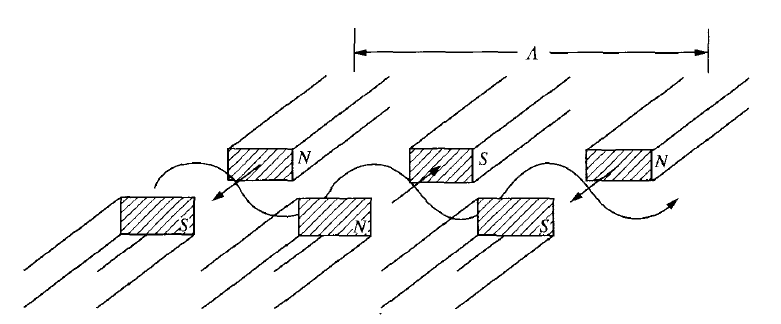
\includegraphics[width=0.75\textwidth]{Undulator}
\caption{Relativisztikus elektronok trajektóriája az undulátorban.}
\end{figure}

\end{document}